% CVPR template (https://github.com/cvpr-org/author-kit), camera-ready style with page numbers.
\documentclass[10pt,twocolumn,letterpaper]{article}
\usepackage[pagenumbers]{cvpr}
\usepackage{graphicx,booktabs,amsmath,amssymb,multirow,xcolor,adjustbox}
\usepackage[T1]{fontenc}
\definecolor{cvprblue}{rgb}{0.21,0.49,0.74}
\usepackage[breaklinks,colorlinks,allcolors=cvprblue]{hyperref}
\hypersetup{pdftitle={Three-Class Diabetic Retinopathy Referral Triage with a Sensitivity Guarantee},
  pdfauthor={Swayam Sahu, Sahil Sihag, Nitesh Kumar},
  pdfsubject={Machine Learning course project, IIT Jodhpur}}
\def\confName{CVPR}
\def\confYear{2027}
\newcommand{\pct}{\,\%}
\setlength{\tabcolsep}{3pt}
\graphicspath{{../figures/}{../results/}}

\title{Three-Class Diabetic Retinopathy Referral Triage\\with a Sensitivity Guarantee}
\author{Swayam Sahu\qquad Sahil Sihag\qquad Nitesh Kumar\\
M.Tech (Data and Computational Sciences), Department of Mathematics, IIT Jodhpur\\
{\tt\small m26mac010@iitj.ac.in \quad m26mac008@iitj.ac.in \quad m24ma2006@iitj.ac.in}\\
{\small Machine Learning course project. Code: \url{https://github.com/Nova1369/dr-triage}}}

\begin{document}
\maketitle

\begin{abstract}
From one fundus photo, our rule decides \emph{no referral}, \emph{routine referral} or \emph{urgent referral}, or passes the eye to a human grader, with a stated promise: at most 10\pct{} of the eyes that need a referral are sent home, and at least 90\pct{} of the urgent eyes are referred urgently. The rule (C1) sets one conformal threshold per class on the probabilities of a logistic regression on frozen ResNet-50 features. On 3,662 APTOS photos it sends home 4.4\pct{} of referable eyes and refers 91.4\pct{} of urgent eyes urgently; the most likely class reaches 11.7\pct{} and 51.0\pct. At a new clinic the promise breaks (Messidor-2: 87.1\pct{} of referable eyes sent home). Setting the three thresholds again on 300 graded local photos (C2) restores both targets at IDRiD and Messidor-2, which retraining the model does not. With fewer sick eyes the promise holds and the workload falls, and the workload can be forecast from photos without labels when only the share of sick eyes changes (C3). Work beyond the proposal shows that a promise per class is not a promise per group of patients: on the APTOS cameras that photographed mostly healthy eyes, 52.7\pct{} of referable eyes are sent home, because the model recognises the camera. Thresholds per $k$-means cluster bring every camera group below 10\pct{} without knowing the camera, at a price that shows what the shortcut was worth. An alarm that needs ten photos without labels warns when a clinic's photos are unlike the calibration photos.
\end{abstract}

\section{Introduction}
About 101 million Indian adults have diabetes~\cite{indiab}, and 12.5\pct{} of them have diabetic retinopathy (DR)~\cite{smart}, which can blind before it is noticed. Graders are scarce, and deep networks grade DR about as well as experts~\cite{gulshan16,gulshan19}. What a screening programme still lacks is a referral rule with a \emph{stated} sensitivity that is checked when the rule moves to another clinic.

We group the five DR grades~\cite{wilkinson} as in the ICO guidelines~\cite{ico}: grades 0--1 \emph{no referral}, grade 2 \emph{routine referral}, grades 3--4 \emph{urgent referral}. The two targets are: at most 10\pct{} of the eyes that need a referral (grades 2--4, ``referable'') are sent home, and at least 90\pct{} of the urgent eyes are referred urgently. An eye the rule cannot decide goes to a human grader.

\textbf{Deliverables of the proposal.} (C1) a referral rule with one conformal threshold per class; (C2) its recalibration at a new clinic with a few graded local photos; (C3) its behaviour and workload when sick eyes are rarer. Experiments E0 (the coverage drop of standard conformal prediction at a new clinic~\cite{hasan}), E1 (the course's models), E2 (new clinics) and E3 (prevalence); baselines B0--B9; further scores, an error analysis, robustness, ablations and $k$-means (Secs.~\ref{sec:data}--\ref{sec:results}).

\textbf{Additional work.} Section~\ref{sec:extra}, kept separate, goes beyond the proposal on one question that came out of the error analysis: the rule keeps its promise on average, but does it keep it for every group of patients, and can a clinic tell without labels that the promise no longer holds?

\section{Related work}
\textbf{Automated DR screening.} Gulshan \etal~\cite{gulshan16} trained a deep network on 128,175 photos and reached an AUC of 0.990 for referable DR on Messidor-2; a similar system matched manual graders at two Indian sites (sensitivity 88.9\pct{} and 92.1\pct)~\cite{gulshan19}. Abr\`amoff \etal\ report a sensitivity of 96.8\pct{} on Messidor-2 at a fixed set point, with a specificity of 59.4\pct~\cite{abramoff13} and, with deep learning, 87.0\pct~\cite{abramoff16}. These papers measure a fixed algorithm at an operating point. We do not compete on accuracy: our model is a frozen network plus logistic regression. Our contribution is the rule on top of it, which turns two targets into a guarantee that we then test at new clinics.

\textbf{Conformal prediction.} Vovk~\cite{vovk} shows that a label-conditional version of inductive conformal prediction controls the error of each class separately; our one threshold per class is of this kind. Hasan \etal~\cite{hasan} is the closest work: they train three networks on APTOS and find that standard conformal predictors, about nominal on APTOS, cover only 66--71\pct{} of IDRiD photos at a 90\pct{} target with EfficientNet-B0 (77\pct{} with their own ordinal score) and 68.4\pct{} with ResNet-50 and the LAC score. They name shift-aware calibration as future work. We differ in three ways: our guarantee is per referral class and tied to clinical targets; we repair the failure with graded local photos; and we forecast the workload. Ahamed \etal~\cite{ahamed} vary the training augmentation on one dataset; we keep the model fixed and vary the clinic.

\textbf{Label shift.} Podkopaev and Ramdas~\cite{podkopaev} adapt conformal prediction to a change in class shares and note that label-conditional thresholds are another route. Saerens \etal~\cite{saerens} estimate new class shares from unlabelled data with EM; we use their estimate to forecast referrals. At our new clinics the photos themselves change as well, which is a different shift.

\section{Data and preprocessing}\label{sec:data}
\begin{table*}[t]\centering\small
\begin{adjustbox}{max width=\linewidth}\begin{tabular}{@{}llrlll@{}}\toprule
Dataset & Site and cameras & Photos & Grades 0/1/2/3/4 & No referral / routine / urgent & Role\\\midrule
APTOS 2019~\cite{aptos} & Aravind Eye Hospital, India; 17 photo sizes & 3,662 & 1,805/370/999/193/295 & 2,175 (59.4\pct) / 999 (27.3\pct) / 488 (13.3\pct) & training, calibration, test\\
IDRiD~\cite{idrid} & eye clinic, Nanded, India; one camera & 516 & 168/25/168/93/62 & 193 (37.4\pct) / 168 (32.6\pct) / 155 (30.0\pct) & new clinic 1\\
Messidor-2~\cite{decenciere,abramoff13} & three French hospitals; three photo sizes & 1,744 & 1,017/270/347/75/35 & 1,287 (73.8\pct) / 347 (19.9\pct) / 110 (6.3\pct) & new clinic 2\\\bottomrule
\end{tabular}\end{adjustbox}
\caption{The 5,922 photos. APTOS test labels were never released, so its 3,662 labelled photos are used with cross-validation. Messidor-2 grades are the adjudicated grades of Krause \etal~\cite{krause} (1,744 gradable photos of 1,748).}\label{tab:data}
\end{table*}
Three public datasets are used (Tab.~\ref{tab:data}); no new data is collected. APTOS trains, calibrates and tests the rule; IDRiD and Messidor-2 play two new clinics and are never used to train or tune the APTOS model. The Messidor-2 licence forbids passing the photos on in any form, so no photo, crop or feature file is in the repository.

Each photo is cropped to the box that contains its retina (pixels brighter than the black background), padded to a square and resized to $224{\times}224$ pixels; colours are not changed. APTOS contains copies of photos, some with different grades. Two photos count as copies when the cosine similarity of their features exceeds 0.995; 270 APTOS photos fall into 131 such groups. APTOS is split into 10 folds with the same mix of grades, and a group of copies is never split across folds.

\section{Method}\label{sec:method}
\textbf{Features and model.} A ResNet-50~\cite{he,timm} pretrained on ImageNet and not trained by us turns each crop into 2,048 features. The features are standardised and reduced to 100 principal components, and the course's models are trained on them with scikit-learn~\cite{sklearn}. Logistic regression is carried forward (Sec.~\ref{sec:e1}).

\textbf{Conformal prediction.} For a calibration photo of class $y$ (a photo with a known label that the model was not trained on) the score is $s=1-\hat p(y\mid x)$~\cite{sadinle}. With $n$ calibration scores, the threshold $\hat q$ is the $\lceil (n+1)(1-\alpha)\rceil$-th smallest, and the prediction set $C(x)=\{c: 1-\hat p(c\mid x)\le \hat q\}$ contains the true class with probability at least $1-\alpha$, provided the new photo is exchangeable with the calibration photos~\cite{vovk,angelopoulos}. We use $\alpha=0.1$.

\textbf{C1: one threshold per class.} Standard conformal prediction (B4) has one threshold, so its 90\pct{} is an average over all eyes, most of which are healthy. C1 sets $\hat q_c$ from the calibration photos of class $c$ only, so $P(c\in C(x)\mid y=c)\ge 1-\alpha$ holds for each class. A class needs at least 9 calibration photos; with fewer the threshold is infinite and the class is always kept. The decision is: \emph{urgent} if urgent is in the set; \emph{routine} if the set is exactly \{routine\}; \emph{no referral} if it is exactly \{no referral\}; otherwise a grader decides. A referable eye is sent home only if its set is exactly \{no referral\}, that is, only if its true class was left out, which happens at most 10\pct{} of the time. An urgent eye is referred urgently whenever urgent is in its set, at least 90\pct{} of the time. These are the two targets.

\textbf{C2: a new clinic.} The APTOS model is kept, and only the three thresholds are set again, on $n$ graded photos of the clinic. The guarantee then holds at that clinic, whatever the quality of the model there.

\textbf{C3: fewer sick eyes.} A threshold looks only at the eyes of its class, so the guarantee does not depend on the class shares~\cite{podkopaev}. The workload does. With $r_y$ the share of class-$y$ eyes the rule refers (measured at APTOS) and $\pi_y$ the clinic's class shares, the forecast is $1000\sum_y \pi_y r_y$ referrals per 1,000 eyes. C3 estimates $\pi$ from the clinic's unlabelled photos with the EM procedure of Saerens \etal~\cite{saerens}.

\textbf{Baselines.} B0 send everyone home / refer everyone urgently; B1 the most likely class; B2 a model that sees only the photo's size, brightness and sharpness, never the retina; B3 two cut-offs on $P(\text{referable})$ and $P(\text{urgent})$ tuned on the calibration photos to catch 90\pct~\cite{gulshan16,abramoff16}; B4 standard conformal prediction~\cite{hasan}; B5 an ``unsure'' band (to a grader if the highest probability is below 0.6); B6 no recalibration at the new clinic; B7 the model retrained with the local photos; B8 the workload forecast with APTOS's class shares; B9 with the true shares (not known in practice).

\textbf{Protocol.} In each of 10 rounds, one APTOS fold is tested, the next fold is the calibration fold, and the model is trained on the other eight. Every APTOS photo is thus decided once, by a model and thresholds that never saw it or a copy of it. Scaling and PCA are fitted on the training folds only. The same 10 models and thresholds are applied to the new clinics. For C2, $n$ local photos are drawn 5 times for each of the 10 models (50 runs), and every rule is tested on the clinic's other photos. Intervals are 95\pct{} bootstrap or Wilson intervals; ranges over runs hold 90\pct{} of the runs.

\section{Results}\label{sec:results}
\subsection{E1: which model reads the features best?}\label{sec:e1}
\begin{table}[t]\centering\small
\begin{adjustbox}{max width=\linewidth}\begin{tabular}{@{}lccc@{}}\toprule
Model & \multicolumn{2}{c}{AUROC} & Accuracy\\
 & referable & urgent & \\\midrule
Logistic regression & 0.972 & 0.917 & 0.825\\
LDA & 0.970 & 0.919 & 0.816\\
SVM (RBF) & 0.970 & 0.910 & 0.824\\
MLP & 0.966 & 0.875 & 0.790\\
Gradient boosting & 0.963 & 0.898 & 0.799\\
$k$-nearest neighbours & 0.957 & 0.878 & 0.774\\
Random forest & 0.953 & 0.891 & 0.777\\
AdaBoost & 0.944 & 0.873 & 0.763\\
QDA & 0.941 & 0.881 & 0.775\\
B2: photo size, brightness, sharpness & 0.921 & 0.782 & 0.725\\
Decision tree & 0.908 & 0.821 & 0.721\\
Naive Bayes & 0.839 & 0.790 & 0.645\\
Class shares only (no photo) & 0.494 & 0.492 & 0.594\\\bottomrule
\end{tabular}\end{adjustbox}
\caption{E1: the course's models on the ResNet-50 features, 3,662 APTOS photos, 10-fold nested cross-validation (settings chosen by an inner 3-fold grid search). Intervals are in \texttt{results/models.csv}.}\label{tab:e1}
\end{table}
Table~\ref{tab:e1} compares eleven models and two reference points. Logistic regression (0.972, 95\pct{} interval 0.968--0.977), LDA and the SVM are within each other's intervals; we carry logistic regression forward because it is the simplest, with $C=0.01$, the setting chosen most often. B2 never sees the retina and still reaches 0.921: in APTOS the camera and the image quality already say a lot about the grade. Section~\ref{sec:extra} returns to this.

\subsection{C1 on APTOS}
\begin{table}[t]\centering\small
\begin{adjustbox}{max width=\linewidth}\begin{tabular}{@{}lrrrrr@{}}\toprule
Rule & \shortstack{Ref.\\home} & \shortstack{Urgent\\urgently} & \shortstack{Healthy\\home} & \shortstack{To a\\grader} & \shortstack{Referrals\\per 1,000}\\\midrule
B1 most likely class & 11.7 & 51.0 & 93.4 & 0.0 & 398\\
B3 tuned cut-offs & 9.0 & 87.9 & 91.0 & 0.0 & 423\\
B4 one threshold & 6.6 & 69.7 & 89.2 & 8.5 & 358\\
B5 unsure band & 7.9 & 39.3 & 90.8 & 14.3 & 286\\
\textbf{C1 (ours)} & \textbf{4.4} & \textbf{91.4} & 87.2 & 1.8 & 446\\\bottomrule
\end{tabular}\end{adjustbox}
\caption{C1 against simpler rules on APTOS, in percent. ``Ref.\ home'': referable eyes sent home (target at most 10). ``Urgent urgently'': urgent eyes referred urgently (target at least 90). The two B0 rules are trivial (100/0 and 0/100).}\label{tab:c1}
\end{table}
Only C1 meets both targets (Tab.~\ref{tab:c1}): it sends home 4.4\pct{} of referable eyes (3.4--5.5) and refers 91.4\pct{} of urgent eyes urgently (88.9--93.8). The most likely class (B1) refers only half of the urgent eyes urgently. With one threshold for all classes (B4), the true class is in the set for 95.9\pct{} of healthy eyes but only 69.7\pct{} of urgent eyes; with one threshold per class the three classes get 90.3\pct, 90.9\pct{} and 91.4\pct. Tuned cut-offs (B3) come close but carry no guarantee and miss the urgent target. The price of C1 is more referrals, 446 per 1,000 eyes, because 68\pct{} of grade-2 eyes are referred urgently to be safe.

\subsection{E0 and E2: the rule at a new clinic}
\begin{table}[t]\centering\small
\begin{adjustbox}{max width=\linewidth}\begin{tabular}{@{}llrrrr@{}}\toprule
Clinic & Rule & \shortstack{True class\\in the set} & \shortstack{Ref.\\home} & \shortstack{Urgent\\urgently} & \shortstack{Referrals\\per 1,000}\\\midrule
APTOS & B4 & 90.3 & 6.6 & 69.7 & 358\\
APTOS & C1 & 90.6 & 4.4 & 91.4 & 446\\
IDRiD & B4 & 76.8 & 16.9 & 58.3 & 391\\
IDRiD & C1 & 82.2 & 13.6 & 87.0 & 578\\
Messidor-2 & B4 & 75.3 & 91.8 & 19.4 & 17\\
Messidor-2 & C1 & 76.3 & 87.1 & 38.9 & 44\\\bottomrule
\end{tabular}\end{adjustbox}
\caption{E0: the APTOS models and thresholds applied unchanged to the new clinics (average of the 10 rounds, percent). The promised 90\pct{} is lost.}\label{tab:e0}
\end{table}
Applied unchanged, both rules lose their promise (Tab.~\ref{tab:e0}). At IDRiD both targets are missed. At Messidor-2 the rule fails completely: the model gives almost every photo a high probability of ``no referral'' (0.96 on average even for grade-2 eyes), so 87.1\pct{} of referable eyes are sent home. The AUROC for referable eyes falls from 0.972 at APTOS to 0.910 at IDRiD and 0.684 at Messidor-2.

The IDRiD row of B4 is our check of Hasan \etal~\cite{hasan} (E0). They report 68.4\pct{} coverage for a ResNet-50 trained on APTOS with the same score; B4, on frozen ResNet-50 features with logistic regression, covers 76.8\pct. We confirm the finding, coverage far below the promised 90\pct; how far it falls depends on the model. They use 455 IDRiD photos and we use all 516, so the numbers are not directly comparable.

\subsection{C2: a few local photos repair the promise}
\begin{table}[t]\centering\small
\begin{adjustbox}{max width=\linewidth}\begin{tabular}{@{}llrrrr@{}}\toprule
Clinic & Rule & \shortstack{True class\\in the set} & \shortstack{Ref.\\home} & \shortstack{Urgent\\urgently} & \shortstack{To a\\grader}\\\midrule
IDRiD & B6 no recalibration & 82.1 & 13.6 & 87.1 & 5.5\\
IDRiD & \textbf{C2 (ours)} & \textbf{90.5} & \textbf{5.7} & \textbf{90.3} & 20.8\\
IDRiD & B7 retrained & 82.4 & 6.8 & 96.6 & 3.3\\
IDRiD & RR retr.\ + recal. & 91.4 & 4.8 & 91.6 & 20.7\\\midrule
Messidor-2 & B6 no recalibration & 76.2 & 87.1 & 38.5 & 0.1\\
Messidor-2 & \textbf{C2 (ours)} & \textbf{90.2} & \textbf{6.5} & \textbf{92.2} & 45.4\\
Messidor-2 & B7 retrained & 80.1 & 46.8 & 71.6 & 8.1\\
Messidor-2 & RR retr.\ + recal. & 90.8 & 2.8 & 95.6 & 19.3\\\bottomrule
\end{tabular}\end{adjustbox}
\caption{E2 with $n=300$ graded local photos (average of 50 runs, percent). RR, not in the proposal, uses half of the local photos to retrain and half to set the thresholds.}\label{tab:c2}
\end{table}
\begin{figure}[t]\centering
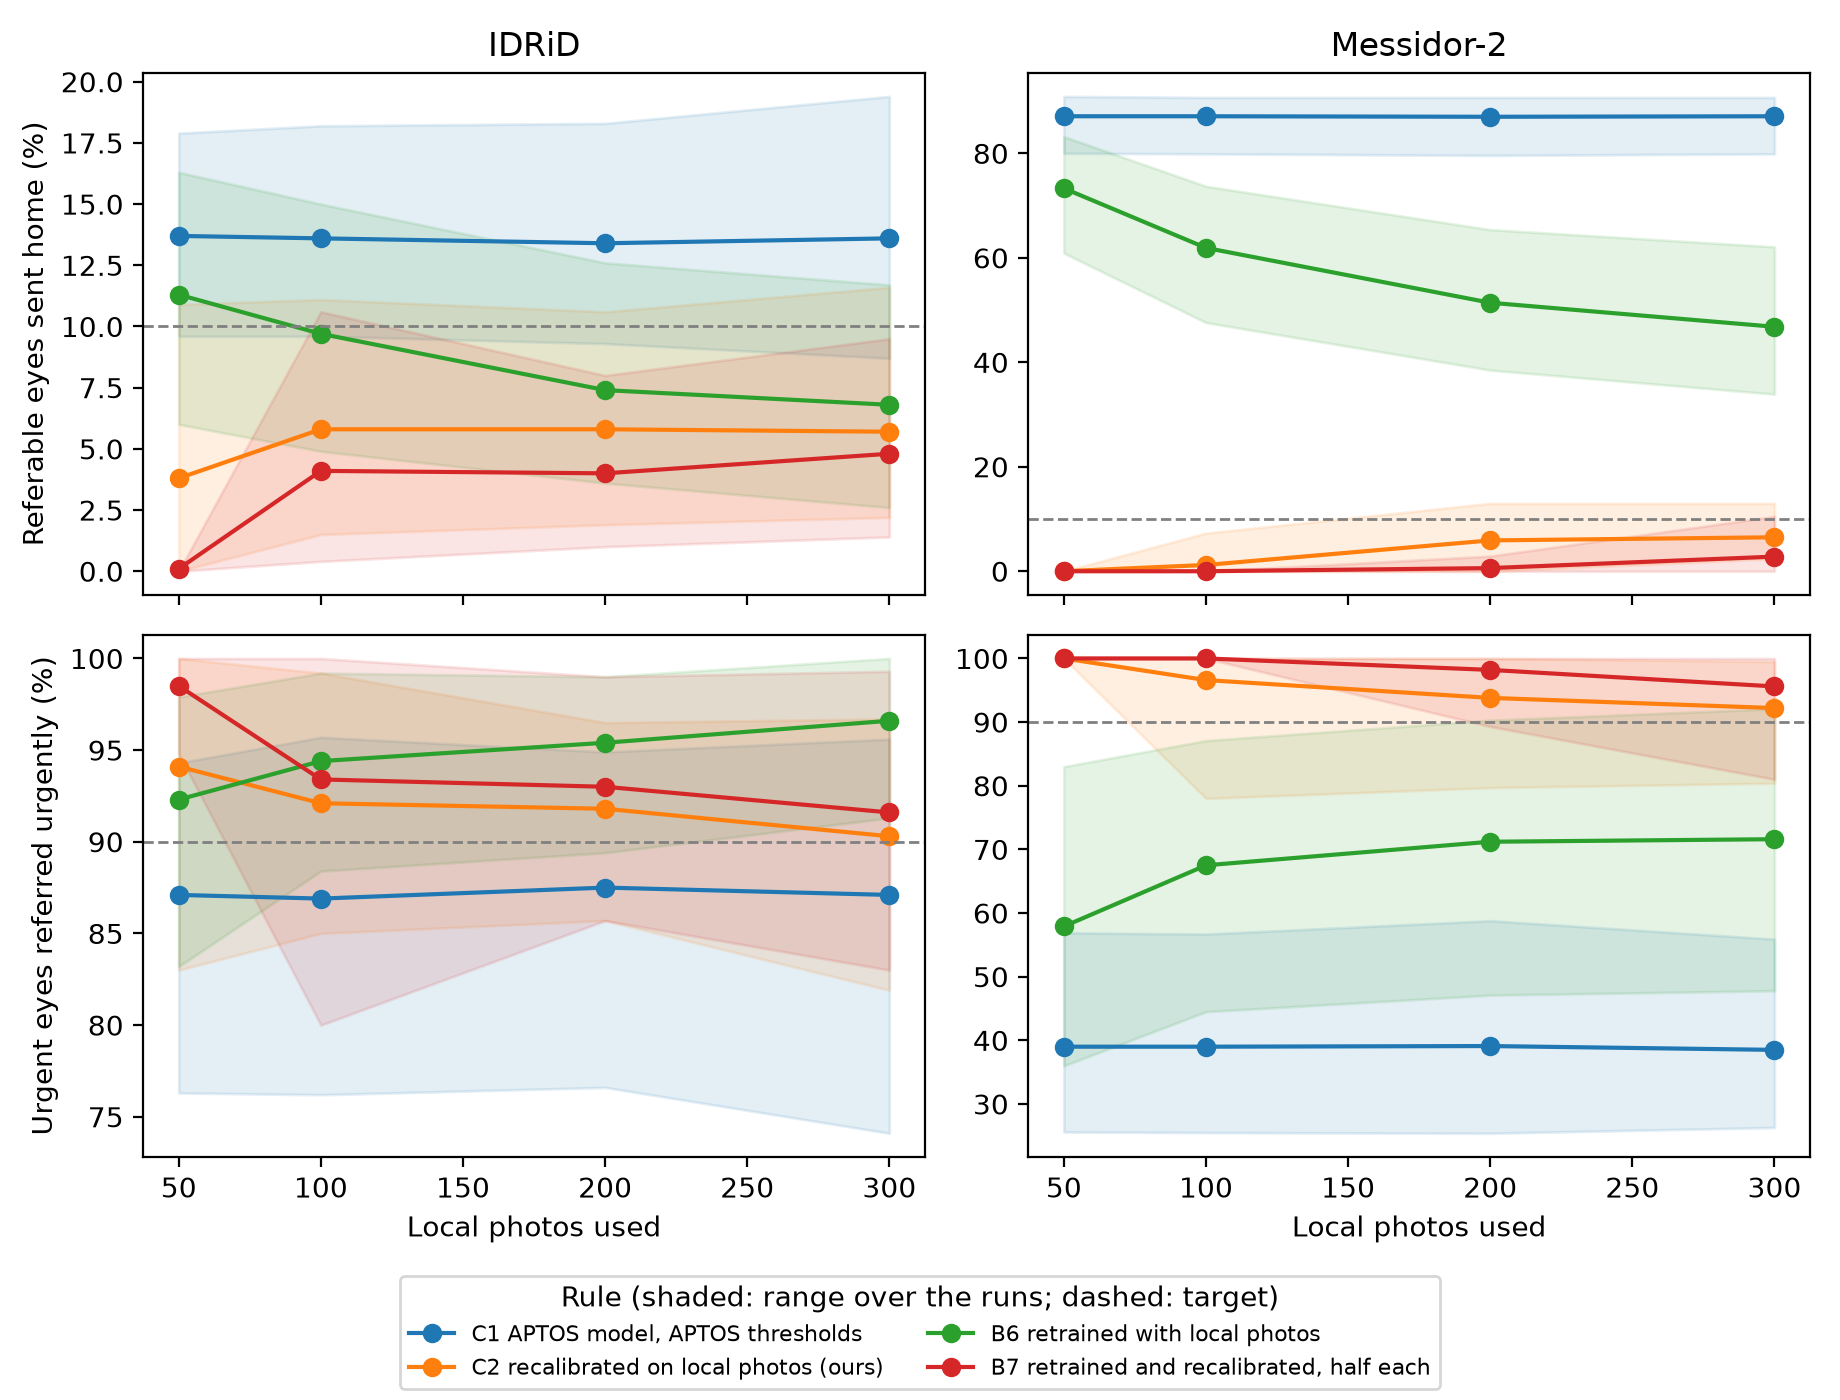
\includegraphics[width=\linewidth]{recalibration_by_clinic.png}
\caption{The four rules against the number of local photos. Lines: average of 50 runs; bands: the range of 90\pct{} of the runs; dashed: the targets.}\label{fig:c2}
\end{figure}
With 300 local photos, setting the thresholds again brings the 90\pct{} back at both clinics, and both targets are met on average, without touching the model (Tab.~\ref{tab:c2}, Fig.~\ref{fig:c2}). Retraining alone (B7) does not: 300 local photos among 2,900 APTOS photos barely move the model, and at Messidor-2 it still sends home 46.8\pct{} of referable eyes. RR also keeps the promise, which shows that what repairs it is where the thresholds are set, not the retraining; RR needs a new model for every clinic.

The guarantee does not make the model better, and the cost shows in the workload. At Messidor-2, where the model ranks eyes poorly, the rule stays safe by being unsure: 45.4\pct{} of the eyes go to a grader. With too few local photos the rule is safe but useless: among 50 Messidor-2 photos there are about 3 urgent eyes, too few for an urgent threshold, so every eye is referred urgently. About 200 to 300 photos are needed there. The numbers are averages; a single draw can land a few points either side of a target (Fig.~\ref{fig:c2}).

\subsection{C3 and E3: fewer sick eyes}
\begin{table}[t]\centering\small
\begin{adjustbox}{max width=\linewidth}\begin{tabular}{@{}rrrrrrr@{}}\toprule
 & \multicolumn{2}{c}{C1} & \multicolumn{2}{c}{B4, in the set} & \multicolumn{2}{c}{C1 referrals}\\
\shortstack{Referable\\eyes} & \shortstack{Ref.\\home} & \shortstack{Urgent\\urgently} & \shortstack{true\\class} & \shortstack{urgent\\eyes} & \shortstack{per\\1,000} & \shortstack{needed}\\\midrule
5 & 4.0 & 91.5 & 95.2 & 70.1 & 151 & 31.1\\
12.5 & 4.5 & 91.2 & 94.2 & 68.4 & 214 & 55.0\\
25 & 4.6 & 91.4 & 92.5 & 69.7 & 316 & 74.2\\
40.6 (APTOS) & 4.4 & 91.6 & 90.3 & 69.7 & 446 & 85.4\\\bottomrule
\end{tabular}\end{adjustbox}
\caption{E3: clinics of 1,000 eyes drawn from APTOS with fewer referable eyes (average of 200 clinics, percent).}\label{tab:e3}
\end{table}
\begin{table}[t]\centering\small
\begin{adjustbox}{max width=\linewidth}\begin{tabular}{@{}lrrrrrr@{}}\toprule
 & \multicolumn{2}{c}{Referable \%} & & \multicolumn{3}{c}{Forecast (average miss)}\\
Clinic & true & est. & Obs. & B8 & C3 (ours) & B9\\\midrule
APTOS, 5\pct & 5.0 & 5.8 & 151 & 445 (294) & 157 (11) & 151 (11)\\
APTOS, 12.5\pct & 12.5 & 13.0 & 214 & 446 (232) & 218 (9) & 213 (11)\\
APTOS, 25\pct & 25.0 & 25.1 & 316 & 447 (132) & 319 (7) & 318 (10)\\
IDRiD & 62.6 & 60.9 & 578 & 446 (131) & 612 (44) & 632 (55)\\
Messidor-2 & 26.2 & 0.3 & 44 & 446 (402) & 113 (69) & 326 (282)\\\bottomrule
\end{tabular}\end{adjustbox}
\caption{Referrals per 1,000 eyes: observed, and forecast with APTOS's class shares (B8), shares estimated from photos without labels (C3) and the true shares (B9).}\label{tab:c3}
\end{table}
In APTOS 40.6\pct{} of the eyes need a referral; in a screening programme it is nearer 5 to 25\pct. The promise of C1 does not move (Tab.~\ref{tab:e3}), because each threshold looks only at the eyes of its class. Standard conformal prediction looks better and better on paper as sick eyes get rarer (95.2\pct{} at 5\pct) while it still covers only 70\pct{} of urgent eyes: one promise for all eyes together is mostly a promise about the healthy ones. What moves is the workload: at 5\pct{} referable eyes C1 makes 151 referrals per 1,000 eyes, and only 31.1\pct{} of them were needed.

When only the share of sick eyes changes, the forecast from photos without labels is as good as with the true shares (off by about 10 referrals per 1,000) and without a correction it is off by up to 294 (Tab.~\ref{tab:c3}). At the real clinics more than the shares has changed. At Messidor-2 the estimate says 0.3\pct{} referable eyes when the truth is 26.2\pct, because the model calls almost every photo healthy; even the true shares give a wrong forecast, because the rule no longer refers each class as often as at APTOS. The estimate is safe to use only after the model has been checked on graded local photos, and those photos then give the shares directly.

\subsection{Further scores and calibration}
\begin{figure}[t]\centering
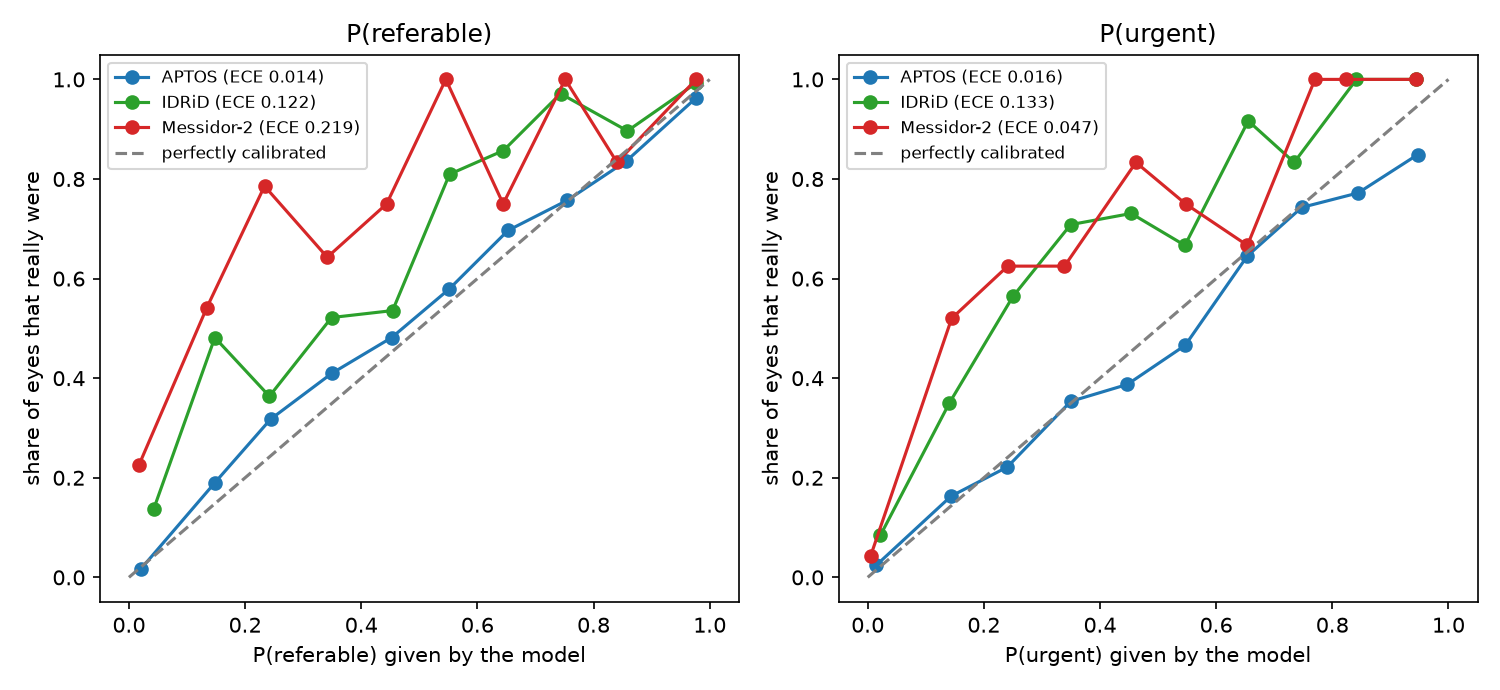
\includegraphics[width=\linewidth]{calibration.png}
\caption{Calibration of the model. A calibrated model stays on the diagonal. At the new clinics the model gives sick eyes too low a risk.}\label{fig:cal}
\end{figure}
\begin{table}[t]\centering\small
\begin{adjustbox}{max width=\linewidth}\begin{tabular}{@{}lccccc@{}}\toprule
 & & & & \multicolumn{2}{c}{ECE of}\\
Photos from & Acc. & QWK & Brier & $P$(ref.) & $P$(urg.)\\\midrule
APTOS, class shares only & 0.594 & 0.000 & 0.555 & 0.000 & 0.000\\
APTOS & 0.823 & 0.781 & 0.247 & 0.014 & 0.016\\
IDRiD & 0.624 & 0.627 & 0.502 & 0.122 & 0.133\\
Messidor-2 & 0.744 & 0.150 & 0.466 & 0.219 & 0.047\\\bottomrule
\end{tabular}\end{adjustbox}
\caption{Accuracy, quadratic weighted kappa (QWK), Brier score and calibration error (ECE, 10 bins). The new clinics are predicted by one model trained on all of APTOS.}\label{tab:scores}
\end{table}
At APTOS the probabilities can be read as risks (ECE 0.014, Tab.~\ref{tab:scores}, Fig.~\ref{fig:cal}); at the new clinics they cannot. Messidor-2 shows why accuracy alone misleads: 74\pct{} of its photos are classified correctly because 74\pct{} of its eyes are healthy and the model calls nearly every eye healthy; the kappa of 0.150 says the agreement is barely better than chance. Per class, C1 raises the sensitivity for urgent eyes from 51.0\pct{} (most likely class) to 91.4\pct, and a ``no referral'' from C1 is right 96.6\pct{} of the time; in exchange only 34.8\pct{} of its urgent referrals are urgent eyes (\texttt{results/per\_class.csv}).

\subsection{Which eyes does the rule get wrong?}\label{sec:errors}
\begin{table}[t]\centering\small
\begin{adjustbox}{max width=\linewidth}\begin{tabular}{@{}lrlrl@{}}\toprule
Group & \shortstack{Ref.\\eyes} & Sent home & \shortstack{Urgent\\eyes} & \shortstack{Not referred\\urgently}\\\midrule
All eyes & 1,487 & 4.4 (3.5--5.6) & 488 & 8.6 (6.4--11.4)\\
Grade 2 & 999 & 5.2 (4.0--6.8) & & \\
Grade 3 & 193 & 1.6 (0.5--4.5) & 193 & 7.3 (4.4--11.8)\\
Grade 4 & 295 & 3.7 (2.1--6.6) & 295 & 9.5 (6.6--13.4)\\
Cameras: mostly healthy & 55 & \textbf{52.7} (39.8--65.3) & 15 & 20.0 (7.0--45.2)\\
Cameras: mixed & 262 & 3.8 (2.1--6.9) & 97 & 11.3 (6.5--19.2)\\
Cameras: mostly sick & 1,170 & 2.3 (1.6--3.3) & 376 & 7.4 (5.2--10.6)\\
Blurriest third & 583 & 4.6 (3.2--6.7) & 216 & 8.8 (5.7--13.3)\\
Middle third & 454 & 6.4 (4.5--9.0) & 146 & 7.5 (4.3--13.0)\\
Sharpest third & 450 & 2.2 (1.2--4.0) & 126 & 9.5 (5.5--15.9)\\\bottomrule
\end{tabular}\end{adjustbox}
\caption{The two errors of C1 on APTOS by group, in percent with 95\pct{} Wilson intervals (both targets: at most 10). APTOS does not name the camera; the photo size stands for it. Cameras are grouped by the share of their eyes that need a referral (under 10\pct, over 50\pct, otherwise mixed).}\label{tab:errors}
\end{table}
The targets hold for each grade and each sharpness third, but not for each camera (Tab.~\ref{tab:errors}). On the cameras that photographed mostly healthy eyes (in practice one camera, $1050{\times}1050$, with 974 photos of which 54 need a referral), more than half of the referable eyes are sent home. The finding is hidden in the overall 4.4\pct{} because these cameras hold only 55 of the 1,487 referable eyes. The 42 missed urgent eyes (25 routine referrals, 14 sent home, 3 to a grader) are confident mistakes, not near misses: their median $P(\text{urgent})$ is 0.043, against 0.538 for the urgent eyes that were caught.

\subsection{Robustness, ablations and a stricter target}
\begin{table}[t]\centering\small
\begin{adjustbox}{max width=\linewidth}\begin{tabular}{@{}llrrrrr@{}}\toprule
\shortstack[l]{Photos\\to decide} & Thresholds & \shortstack{In the\\set} & \shortstack{Ref.\\home} & \shortstack{Urgent\\urgently} & \shortstack{Healthy\\home} & \shortstack{To a\\grader}\\\midrule
Original & original & 90.6 & 4.4 & 91.4 & 87.2 & 1.8\\
Blurred & original & 78.8 & 11.8 & 88.9 & 75.4 & 1.6\\
Blurred & recalibrated & 90.4 & 4.2 & 91.2 & 59.3 & 13.1\\
Half brightness & original & 90.2 & 8.9 & 86.7 & 89.4 & 2.9\\
Half brightness & recalibrated & 90.6 & 5.8 & 91.2 & 86.9 & 2.3\\
JPEG quality 20 & original & 67.2 & 14.9 & 86.7 & 66.8 & 1.0\\
JPEG quality 20 & recalibrated & 90.6 & 4.2 & 90.8 & 38.6 & 20.8\\\bottomrule
\end{tabular}\end{adjustbox}
\caption{Worse test photos on APTOS (percent). ``Recalibrated'': thresholds set on calibration photos that are worse in the same way.}\label{tab:robust}
\end{table}
\begin{table}[t]\centering\small
\begin{adjustbox}{max width=\linewidth}\begin{tabular}{@{}lrrrrr@{}}\toprule
Variant & \shortstack{AUROC\\ref.} & \shortstack{Ref.\\home} & \shortstack{Urgent\\urgently} & \shortstack{Healthy\\home} & \shortstack{To a\\grader}\\\midrule
As it is (PCA 100, $C=0.01$) & 0.972 & 4.4 & 91.4 & 87.2 & 1.8\\
PCA with 20 components & 0.958 & 5.9 & 91.0 & 85.3 & 4.3\\
PCA with 300 components & 0.973 & 3.6 & 90.6 & 85.1 & 2.5\\
No PCA (2,048 features) & 0.973 & 2.9 & 92.0 & 83.7 & 3.1\\
No standardising & 0.965 & 5.0 & 90.4 & 87.4 & 2.3\\
Weaker regularisation ($C=1$) & 0.971 & 4.6 & 90.6 & 86.9 & 1.9\\
Half of the training photos & 0.967 & 4.8 & 90.4 & 85.6 & 2.5\\
A tenth of the training photos & 0.954 & 2.8 & 92.6 & 75.4 & 4.5\\\midrule
$\alpha=20$\pct & & 2.2 & 79.7 & 80.3 & 9.1\\
$\alpha=10$\pct{} (ours) & & 4.4 & 91.4 & 87.2 & 1.8\\
$\alpha=5$\pct & & 2.0 & 95.9 & 80.6 & 6.0\\
$\alpha=2$\pct & & 0.4 & 98.4 & 36.3 & 9.6\\\bottomrule
\end{tabular}\end{adjustbox}
\caption{Top: one part of the pipeline changed at a time. Bottom: other allowed miss rates $\alpha$. APTOS, percent.}\label{tab:abl}
\end{table}
\textbf{Worse photos} break the promise in the same way a new clinic does (Tab.~\ref{tab:robust}): blur (radius 1.3 pixels) and JPEG compression miss both targets, and half brightness misses the urgent target although it barely changes the ranking (AUROC 0.966). Thresholds set on equally poor photos bring both targets back every time, at the cost of usefulness: with compressed photos only 38.6\pct{} of healthy eyes are sent home.

\textbf{Ablations} (Tab.~\ref{tab:abl}, top). No single part matters much, and every variant meets both targets, because the guarantee does not depend on how good the model is. A weaker model pays in workload: with a tenth of the training photos (about 290), the rule sends home 75.4\pct{} of the healthy eyes instead of 87.2\pct.

\textbf{A stricter target} (Tab.~\ref{tab:abl}, bottom). $\alpha=5$\pct{} is affordable: 95.9\pct{} of urgent eyes are referred urgently for 6.0\pct{} of eyes to a grader. At 2\pct{} the rule stops being useful. At 20\pct{} many sets are empty, and an empty set also goes to a grader.

\subsection{Do the photos group by grade or by camera?}\label{sec:kmeans}
\begin{figure*}[t]\centering
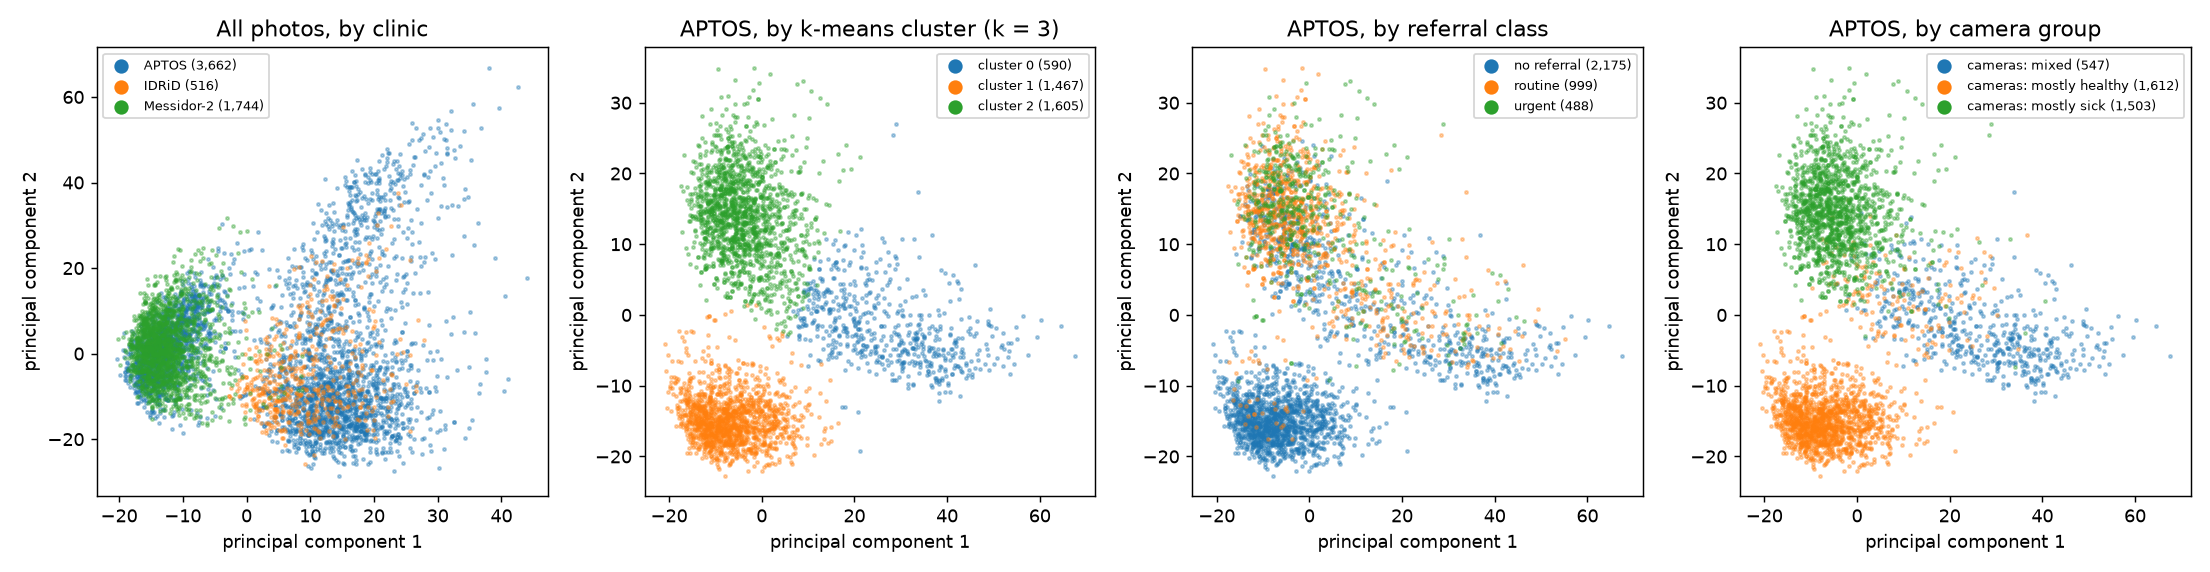
\includegraphics[width=\linewidth]{clusters.png}
\caption{The photos on the first two principal components of their features. The $k$-means clusters of APTOS (second panel) are almost exactly its camera groups (fourth panel), not its referral classes (third panel).}\label{fig:clusters}
\end{figure*}
$k$-means is given the features and nothing else. For APTOS with $k=3$, the clusters agree with the three camera groups of Tab.~\ref{tab:errors} (adjusted Rand index 0.828) far more than with the referral class (0.263) or the DR grade (0.384); see Fig.~\ref{fig:clusters}. Across the three datasets, 1,728 of the 1,744 Messidor-2 photos fall in one cluster and 454 of the 516 IDRiD photos in another. What the frozen network describes first is how a photo was taken. This explains why a model on these features can use the camera as a shortcut~\cite{geirhos} and why it does not carry over to another clinic.

\section{Additional work (beyond the proposal)}\label{sec:extra}
Everything up to here was promised in the proposal. This section is additional. It investigates one Responsible-AI question in depth, \emph{does the guarantee hold for every group of patients?}, proposes two extensions, and tests each against baselines and across the three datasets.

\subsection{The camera shortcut}
Three tests show that the model uses the camera. (a) A logistic regression reads the camera from the features: 94.3\pct{} correct for 13 cameras, against 26.7\pct{} for always guessing the most common one. (b) The same grade gets a different answer on a different camera: a grade-2 eye receives an average $P(\text{no referral})$ of 0.74 on the mostly-healthy cameras and 0.20 and 0.15 on the others. (c) The model ranks eyes less well inside a camera group (AUROC 0.910, 0.964 and 0.885) than over all photos (0.971): part of the 0.971 comes from telling cameras apart, not eyes.

\subsection{A guarantee for each group}
\begin{table}[t]\centering\small
\begin{adjustbox}{max width=\linewidth}\begin{tabular}{@{}lrrrrrr@{}}\toprule
 & \multicolumn{3}{c}{Ref.\ home, cameras} & & & \\
Rule & \shortstack{mostly\\healthy} & mixed & \shortstack{mostly\\sick} & \shortstack{Urgent\\urgently} & \shortstack{Healthy\\home} & \shortstack{To a\\grader}\\\midrule
C1 & \textbf{52.7} & 4.6 & 2.7 & 91.0 & 87.4 & 1.8\\
Per camera group & 3.6 & 3.4 & 3.8 & 90.4 & 57.2 & 20.8\\
\textbf{Per cluster (ours)} & \textbf{3.6} & 3.8 & 4.0 & 90.0 & 60.2 & 18.6\\
Reweighted model & 0.0 & 1.1 & 3.0 & 90.6 & 58.4 & 18.6\\
No home from cluster & 0.0 & 4.6 & 2.7 & 91.0 & 22.9 & 40.9\\\bottomrule
\end{tabular}\end{adjustbox}
\caption{Five rules judged camera group by camera group (APTOS, percent). Three folds are used for calibration here, so C1 differs slightly from Tab.~\ref{tab:c1}. Intervals for the mostly-healthy cameras: 52.7 (39.8--65.3), 3.6 (1.0--12.3), 0.0 (0.0--6.5).}\label{tab:groups}
\end{table}
\begin{figure}[t]\centering
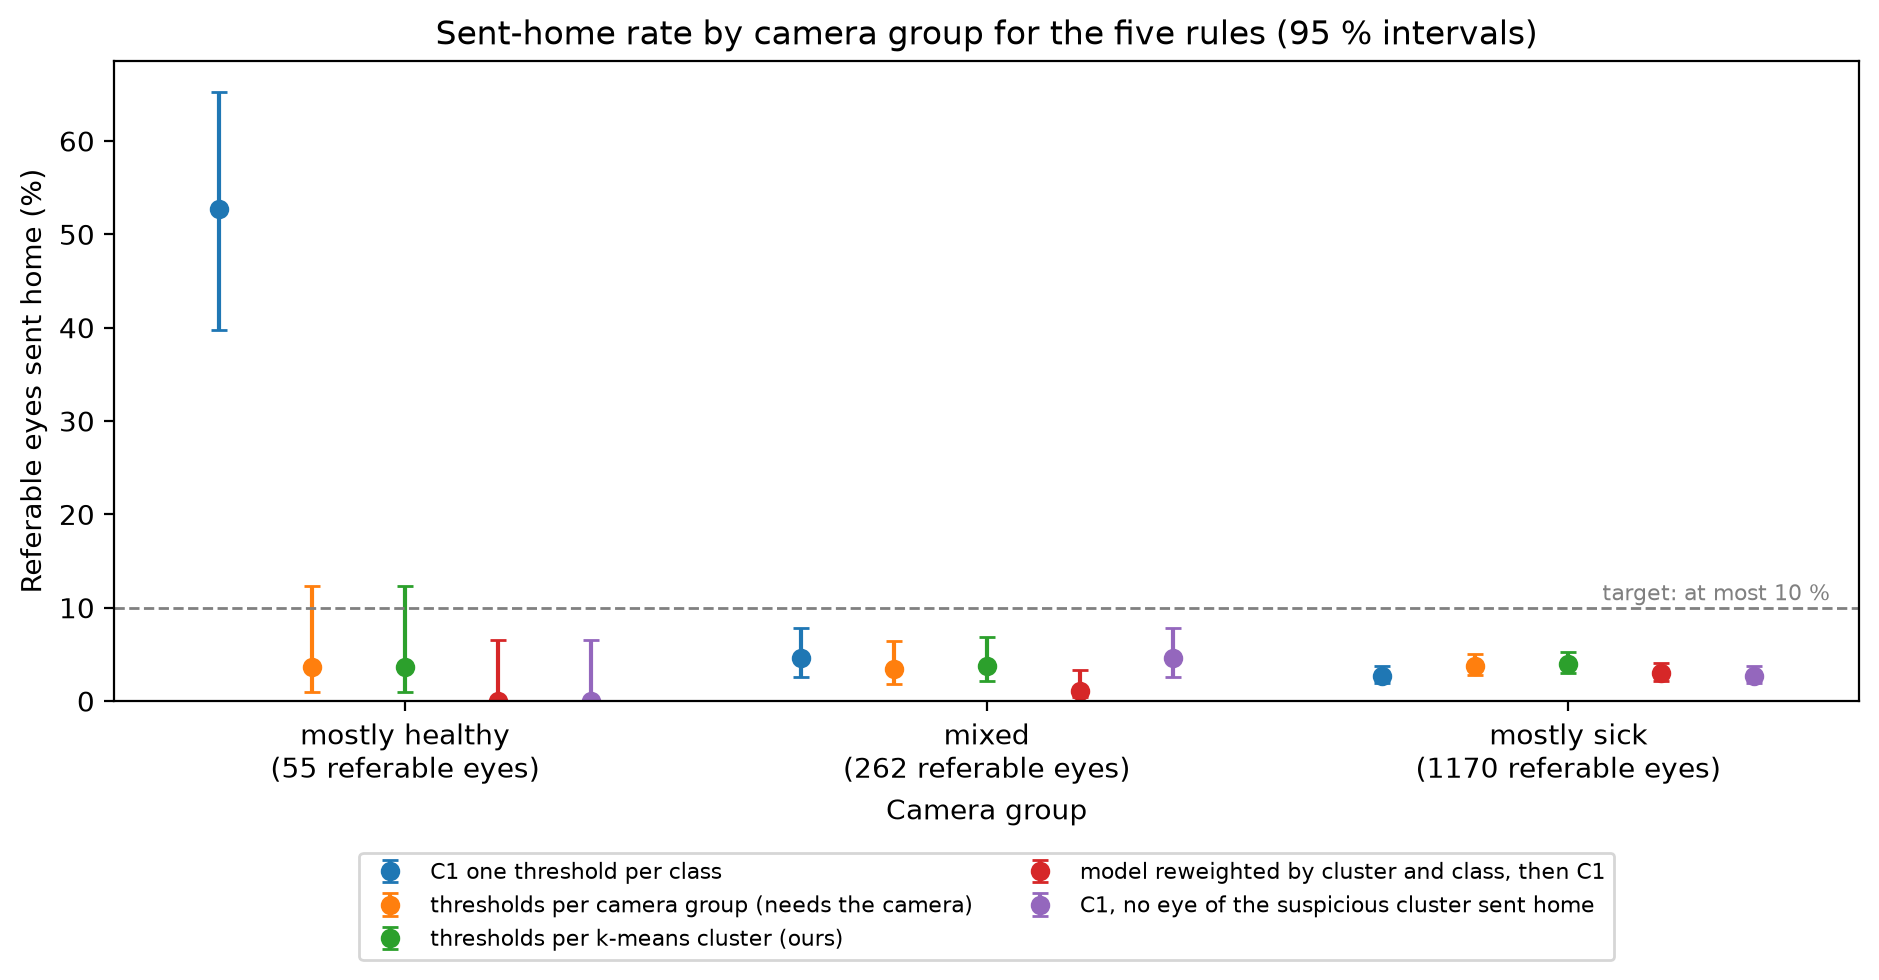
\includegraphics[width=\linewidth]{rules_by_camera_group.png}
\caption{Referable eyes sent home by camera group for the five rules of Tab.~\ref{tab:groups}, with 95\pct{} intervals.}\label{fig:groups}
\end{figure}
Conformal prediction promises an average over the eyes of a class. To keep the promise for each group, we set one threshold per class \emph{and per group}, where the groups are the $k$-means clusters of Sec.~\ref{sec:kmeans}: no camera information and no labels are needed to form them. We compare with thresholds per known camera group (the best case), with a standard way to remove a shortcut (the model retrained with every pair of cluster and class counting the same~\cite{idrissi}, then C1), and with a simple safe rule (no eye of the cluster with the fewest referable eyes is sent home by the rule). A class with fewer than 9 calibration photos in a group keeps the threshold of all groups.

Table~\ref{tab:groups} and Fig.~\ref{fig:groups} give three findings. \emph{First}, the promise can be kept for each group without knowing the camera: the clusters match the camera groups (adjusted Rand index 0.83 on the test folds), and thresholds per cluster do as well as thresholds per known camera. \emph{Second}, the fix has a real price, and the price shows what the shortcut was worth: every rule that protects the troubled cameras sends home about 60\pct{} of the healthy eyes instead of 87\pct{} and passes about 19\pct{} of the eyes to a grader instead of 2\pct. C1 sent home 99\pct{} of the healthy eyes of those cameras, mostly by recognising the camera; part of the usefulness measured on APTOS was the shortcut. \emph{Third}, changing the thresholds and retraining without the shortcut cost about the same, but ours leaves the model alone, so a clinic can apply it with calibration photos only. The simple safe rule is far more expensive (40.9\pct{} to a grader).

\subsection{An alarm for a new clinic}
\begin{table}[t]\centering\small
\begin{adjustbox}{max width=\linewidth}\begin{tabular}{@{}llcrrrr@{}}\toprule
 & & & \multicolumn{2}{c}{Classifier} & \multicolumn{2}{c}{Distance}\\
Photos to decide & \shortstack{Rule\\holds?} & AUROC & $m{=}10$ & 50 & $m{=}10$ & 50\\\midrule
APTOS, fresh & yes & 0.51 & 1 & 0 & 0 & 0\\
APTOS, 5\pct{} referable & yes & 0.58 & 2 & 0 & 0 & 0\\
IDRiD & no & 0.99 & 100 & 100 & 26 & 97\\
Messidor-2 & no & 0.98 & 100 & 100 & \textbf{0} & \textbf{0}\\
APTOS, blurred & no & 1.00 & 100 & 100 & 100 & 100\\
APTOS, half brightness & no & 0.88 & 51 & 100 & 2 & 4\\
APTOS, JPEG quality 20 & no & 1.00 & 100 & 100 & 100 & 100\\\bottomrule
\end{tabular}\end{adjustbox}
\caption{How often each alarm rings (percent of 200 draws) when given $m$ photos without labels. An alarm should ring exactly where C1 misses a target.}\label{tab:alarm}
\end{table}
At Messidor-2 the unchanged rule sends home 87.1\pct{} of referable eyes and nothing warns the clinic, which has no labels when it starts. We test two alarms that get only $m$ unlabelled photos of the clinic. The \emph{distance} alarm, the obvious idea, asks whether the clinic's photos are farther from the APTOS training photos than the calibration photos are (distance to the fifth nearest neighbour, Mann--Whitney test, $p<0.01$). The \emph{classifier} alarm (ours, a classifier two-sample test~\cite{lopezpaz,rabanser}) asks whether a logistic regression can tell the clinic's photos from the calibration photos; it rings when the cross-validated AUROC is at least 0.80.

The classifier alarm rings with ten photos at both clinics and for blurred or compressed photos, needs about 50 for dark photos, and stays silent on fresh APTOS photos (Tab.~\ref{tab:alarm}). It does not ring when only the share of sick eyes changes, which is right: the guarantee holds there (Tab.~\ref{tab:e3}). The distance alarm misses the worst case. Messidor-2 photos are not far from APTOS photos; they sit among APTOS's healthy photos (Fig.~\ref{fig:clusters}), so a distance sees nothing unusual while the rule fails completely.

\textbf{A procedure for a new clinic.} Together with C2 and C3: collect a few photos and run the alarm; if it rings, grade about 300 local photos and set the thresholds again; check the groups; then forecast the workload.

\textbf{Across datasets.} After recalibration with 300 photos, the three cameras of Messidor-2 are treated alike (6.5\pct, 6.1\pct{} and 6.8\pct{} of referable eyes sent home), and thresholds per camera change nothing. The group problem is not a property of the method. It appears in APTOS because there the camera and the grade go together, so it has to be checked at each clinic.

\subsection{How many calibration photos does a group need?}
\begin{figure}[t]\centering
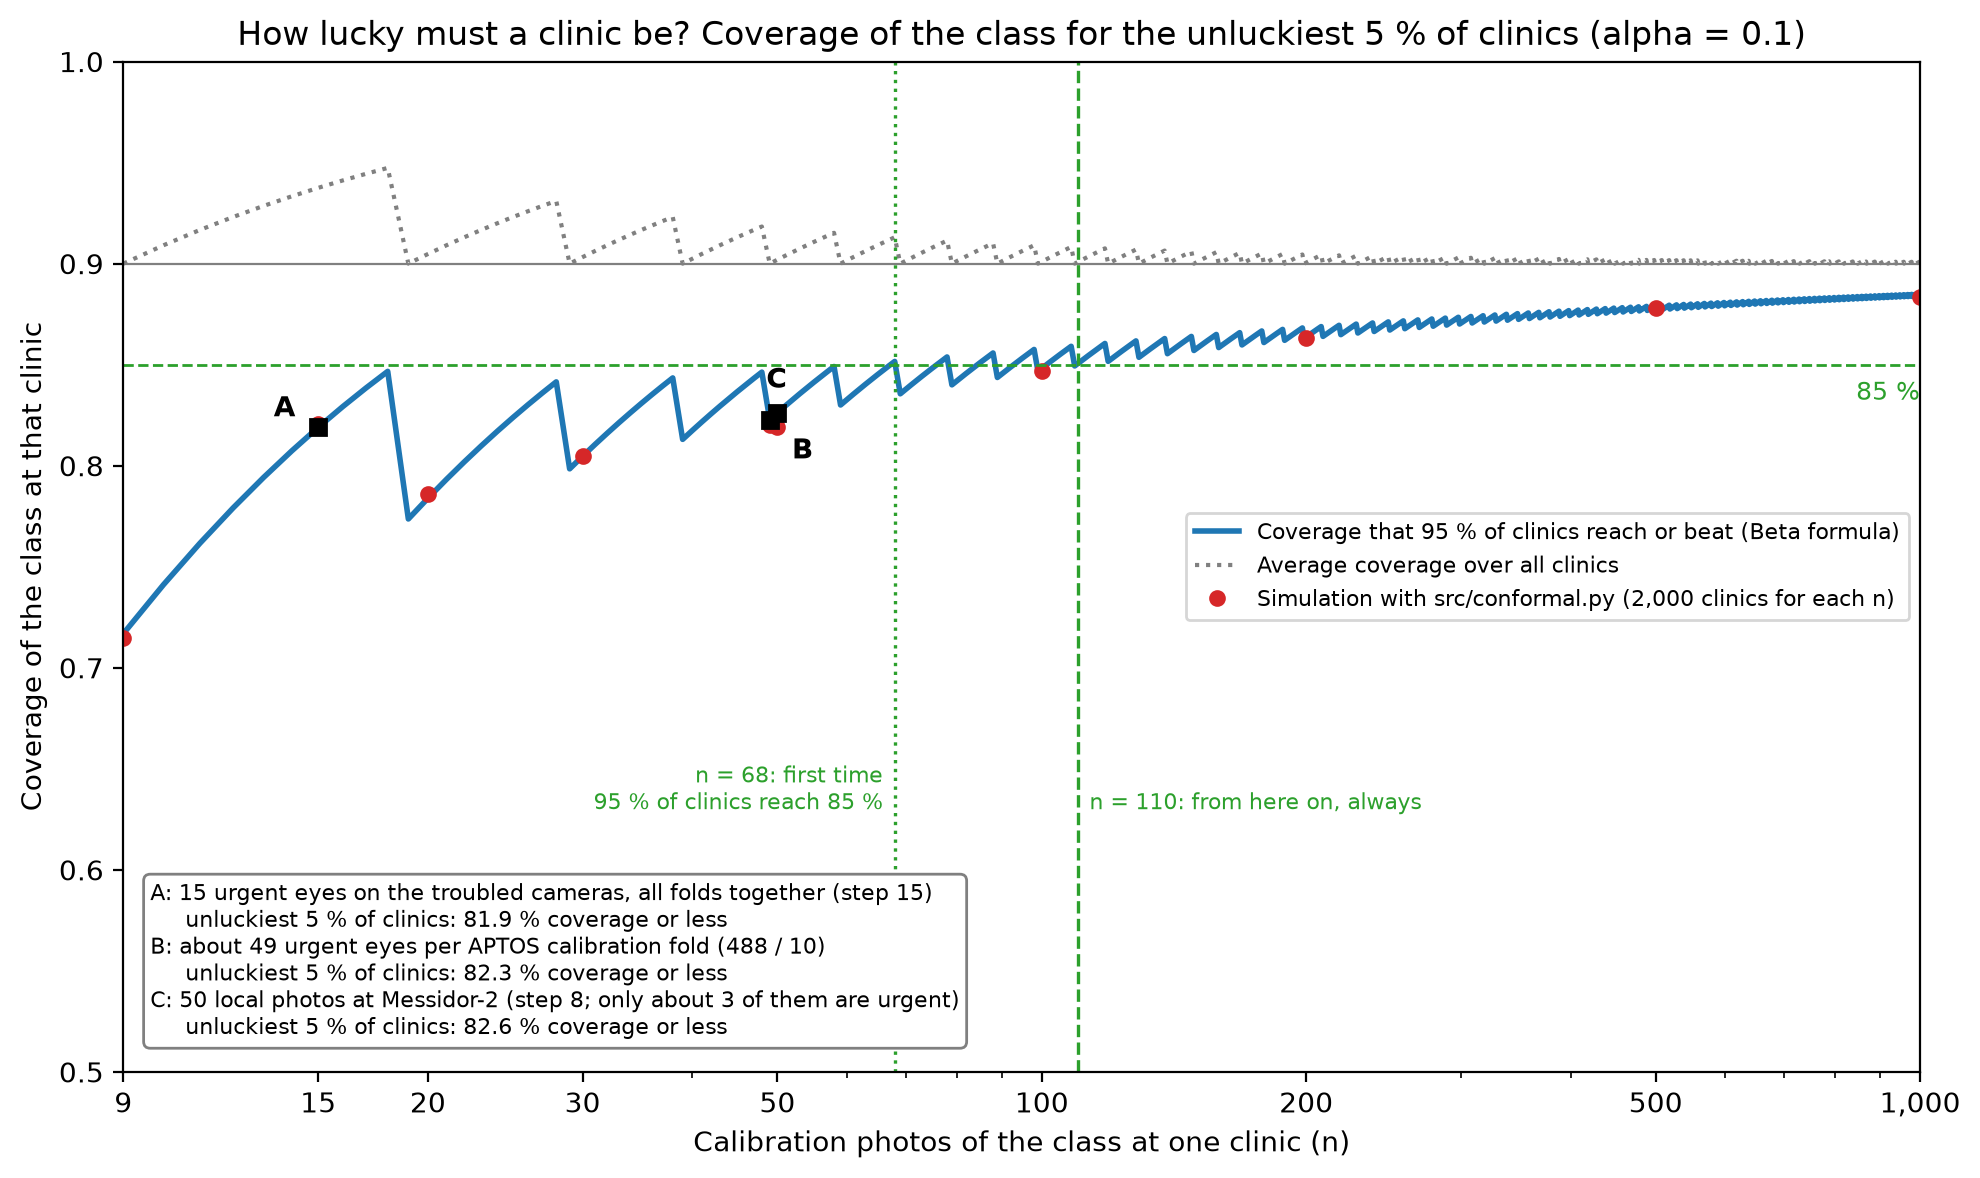
\includegraphics[width=\linewidth]{calibration_size.png}
\caption{Coverage of a class for the unluckiest 5\pct{} of clinics against the number of calibration photos of that class (Beta formula, checked by simulation). A, B, C: class sizes in our experiments.}\label{fig:size}
\end{figure}
The promise holds on average over calibration sets; one clinic has one set. With $n$ calibration photos of a class, the coverage of one clinic follows a Beta$(l,\,n+1-l)$ distribution with $l=\lceil (n+1)(1-\alpha)\rceil$~\cite{vovk,angelopoulos}. Figure~\ref{fig:size} shows the coverage that 95\pct{} of clinics reach: it first exceeds 85\pct{} at $n=68$ and stays above it from $n=110$. The troubled cameras hold 15 urgent eyes in all of APTOS, where the unluckiest 5\pct{} of clinics would get 81.9\pct{} or less. This is the practical limit of a guarantee per group: it needs enough calibration photos of each class in each group.

\subsection{Limits of the additional work}
The troubled cameras have 55 referable eyes, so 3.6\pct{} is 2 eyes and its interval reaches 12.3\pct; their urgent threshold cannot be set and falls back to the threshold of all groups. Cameras are known only through the photo size. The alarm's threshold of 0.80 was chosen on these datasets, and the alarm was tried on two clinics and three kinds of worse photos, not on a clinic whose photos differ only slightly.

\section{Discussion and limitations}
One threshold per class is what makes the guarantee clinical: one threshold for all eyes refers only 69.7\pct{} of urgent eyes urgently. The guarantee belongs to the calibration photos, not to the model: it survives a weaker model, fewer sick eyes and a stricter target, and it is lost with a new clinic, worse photos or a camera the model has learnt, until the thresholds are set again. Safety is paid for with workload, most of all where the model is weak.

\textbf{Limitations.} The frozen ImageNet features rank eyes poorly at Messidor-2 (AUROC 0.684), which caps usefulness there; fine-tuning on fundus photos is the main next step. The guarantee is an average over calibration draws and over the eyes of a class. APTOS has no patient identifiers, so two eyes of one person may fall in different folds. Labels are DR grades only; macular oedema is not part of the decision. Only three public datasets were used, with no prospective study. The model card in the repository (\texttt{report/model\_card.md}) states the intended use and these limits.

\textbf{Changes from the proposal.} Crops are 224 pixels, not 512 (the input size of the network; features of all photos in minutes on a laptop). Calibration uses one fold in each round instead of a fixed 15\pct. Recalibration uses $n=50$ to 300 instead of $k=10$ to 200, because a threshold needs 9 photos of its class. E2 uses the 10 fold models with 5 draws each instead of one model with 200 repeats. The proposal's ``66--77\pct'' for~\cite{hasan} is corrected to 66--71\pct{} for the standard scores. RR is an added rule.

\section{Reproducibility}
\textbf{Declaration.} Every number, table and figure in this report was produced by the code at \url{https://github.com/Nova1369/dr-triage}, at the commits of Tab.~\ref{tab:commits}, from the public datasets, without manual editing. \texttt{bash run\_all.sh} runs the 17 steps in order (about 50 minutes on a laptop, no GPU). A test (\texttt{tests/test\_results.py}) checks the numbers quoted in the README against the tables in \texttt{results/}.

\textbf{Details.} \texttt{requirements.txt} pins the versions (Python 3.13, numpy 2.5.3, pandas 3.0.5, scikit-learn 1.9.1, scipy 1.18.1, torch 2.7.1 for the features). The ResNet-50 weights are checked by their SHA-256. Every script that draws random numbers uses the seed 42. The final model is saved as seven arrays of numbers (\texttt{models/referral\_rule.npz}, 0.8\,MB), and \texttt{src/decide.py} applies them to a photo with numpy only. The photos, crops and features are not in the repository (dataset licences); steps 1 to 4 rebuild them. On another computer the last digit of a number can differ: training the same model on the same photos in a different order moved one urgent eye across its threshold (91.2\pct{} against 91.4\pct), which the test caught.

% Written by report/make_commit_table.py from git log. Do not edit by hand.
\begin{table*}[t]\centering
\begin{minipage}[t]{0.495\textwidth}\centering\scriptsize
\begin{tabular}{@{}r@{\hspace{3pt}}l@{\hspace{3pt}}l@{\hspace{3pt}}l@{\hspace{3pt}}p{0.53\linewidth}@{}}\toprule
\# & Commit & By & Date & Message\\\midrule
1 & \texttt{28b0c75} & Swayam & 12 Nov 18:09 & Project setup: README, requirements, .gitignore\\
2 & \texttt{cf9906e} & Swayam & 12 Nov 18:09 & Step 1: one table of all photos with grade and referral class\\
3 & \texttt{f651a8a} & Swayam & 12 Nov 18:10 & Step 2: crop photos to the retina and resize to 224 px\\
4 & \texttt{3e2af60} & Swayam & 12 Nov 18:10 & Step 3: ResNet-50 features for every photo\\
5 & \texttt{bde8749} & Swayam & 12 Nov 18:10 & Step 4: find copies of the same photo and make 10 folds\\
6 & \texttt{c113820} & Swayam & 13 Nov 17:44 & Step 5: compare the course's models with nested cross-validation\\
7 & \texttt{ad2a54b} & Swayam & 13 Nov 17:44 & Model comparison results; README: step 5 and results so far\\
8 & \texttt{d80d411} & Swayam & 13 Nov 17:44 & The conformal referral rule in its own file, with a self-check\\
9 & \texttt{35d5bec} & Swayam & 14 Nov 11:18 & Step 6: the referral rule on APTOS against simpler rules\\
10 & \texttt{27dc994} & Swayam & 14 Nov 11:18 & Referral rule results; README: step 6\\
11 & \texttt{c1287d7} & Swayam & 14 Nov 20:29 & Step 7: the APTOS rule, unchanged, at IDRiD and Messidor-2\\
12 & \texttt{2d86b09} & Swayam & 14 Nov 20:29 & New-clinic results; README: step 7\\
13 & \texttt{10e484d} & Swayam & 15 Nov 12:06 & Step 8: recalibrate with a few local photos, against retraining\\
14 & \texttt{b60378c} & Swayam & 15 Nov 12:06 & Recalibration results; README: step 8\\
15 & \texttt{fa79f9b} & Swayam & 16 Nov 22:12 & Step 9: the rule at clinics with fewer sick eyes, and a workload forecast\\
16 & \texttt{20e1ee9} & Swayam & 16 Nov 22:12 & Fewer-sick-eyes results; README: step 9\\
17 & \texttt{6aa9385} & Swayam & 17 Nov 22:48 & Step 10: the rule's errors by grade, camera and sharpness\\
18 & \texttt{1d7b5a6} & Swayam & 17 Nov 22:48 & Error analysis results; README: step 10\\
19 & \texttt{ba291dc} & Swayam & 20 Nov 20:20 & Step 11: kappa, Brier score, calibration and per-class scores\\
20 & \texttt{58d7b9d} & Swayam & 20 Nov 20:20 & More scores and calibration chart; README: step 11 and the E0 reproduction\\
21 & \texttt{f7a0fb0} & Swayam & 21 Nov 19:19 & Step 12: features of blurred, dark and compressed photos\\
22 & \texttt{6bac5c7} & Swayam & 21 Nov 19:19 & Step 13: robustness, ablations and other targets\\
\bottomrule
\end{tabular}
\end{minipage}\hfill
\begin{minipage}[t]{0.495\textwidth}\centering\scriptsize
\begin{tabular}{@{}r@{\hspace{3pt}}l@{\hspace{3pt}}l@{\hspace{3pt}}l@{\hspace{3pt}}p{0.53\linewidth}@{}}\toprule
\# & Commit & By & Date & Message\\\midrule
23 & \texttt{10e7a18} & Swayam & 21 Nov 19:19 & Robustness, ablation and target results; README: steps 12 and 13\\
24 & \texttt{4087296} & Sahil & 21 Nov 23:35 & Add pytest tests for the conformal rule\\
25 & \texttt{82e0509} & Sahil & 21 Nov 23:44 & Add report figures script and figures\\
26 & \texttt{40155f7} & Sahil & 22 Nov 23:34 & Fix the pytest version in requirements.txt\\
27 & \texttt{3c04263} & Sahil & 22 Nov 23:43 & Add related work\\
28 & \texttt{cbe02ad} & Swayam & 22 Nov 23:50 & README: correct the comparison with Hasan et al. (E0)\\
29 & \texttt{4fef8f4} & Swayam & 23 Nov 00:01 & Step 14: k-means clusters against grade, camera and clinic\\
30 & \texttt{95d529a} & Swayam & 23 Nov 00:02 & Cluster results and chart; README: step 14\\
31 & \texttt{acee9a7} & Swayam & 23 Nov 13:41 & Additional work, step 15: the camera shortcut and thresholds per group\\
32 & \texttt{ac30ccd} & Swayam & 23 Nov 13:41 & Camera shortcut results; README: additional work, part A\\
33 & \texttt{96066d9} & Sahil & 23 Nov 17:35 & Related work: Messidor-2 note, baseline comparison, small-sample caveat\\
34 & \texttt{4864b36} & Swayam & 24 Nov 02:38 & Additional work, step 16: an alarm for a new clinic\\
35 & \texttt{f364b3c} & Swayam & 24 Nov 02:38 & Alarm results; README: additional work, part B\\
36 & \texttt{bea642a} & Swayam & 24 Nov 11:28 & Step 17: the saved model, and decide.py for single photos\\
37 & \texttt{2b492c5} & Swayam & 24 Nov 11:28 & run\_all.sh; README: saved model, reproducibility, layout\\
38 & \texttt{d19bad0} & Sahil & 24 Nov 18:50 & Add robustness, ablation and group figures, calibration size, model card, results check\\
39 & \texttt{e3f7064} & Sahil & 24 Nov 23:38 & Model card: the alarm of step 16, clearer class size\\
40 & \texttt{6b2c5a2} & Swayam & 25 Nov 00:16 & Baseline names matched to the proposal (B1, B6, B7; RR is new)\\
41 & \texttt{3a646d7} & Swayam & 25 Nov 00:16 & Step 13: shuffle the training photos only when fewer are used\\
42 & \texttt{51fe886} & Swayam & 25 Nov 00:16 & README: names and numbers matched to the tables, changes from the proposal; model card wording\\
43 & \texttt{402a906} & Sahil & 25 Nov 00:21 & Figures redrawn with the final baseline names\\
44 & \texttt{2905464} & Sahil & 25 Nov 01:16 & Model card numbers matched to the final tables\\
\bottomrule
\end{tabular}
\end{minipage}
\caption{Commit history of the repository up to the writing of this report (branch \texttt{main}, 2026, times in IST): the 44 commits that change files. 8 further commits change no file and are not listed.}\label{tab:commits}
\end{table*}


\textbf{Acknowledgement.} Messidor-2 images: Kindly provided by the Messidor program partners (see \url{https://www.adcis.net/en/third-party/messidor/}). Messidor-2 grades: Krause \etal~\cite{krause}.

{\small
\begin{thebibliography}{99}\setlength{\itemsep}{0pt}
\bibitem{aptos} APTOS 2019 Blindness Detection. Kaggle, 2019.
\bibitem{idrid} P.~Porwal \etal. Indian Diabetic Retinopathy Image Dataset (IDRiD). \emph{Data}, 3(3):25, 2018.
\bibitem{decenciere} E.~Decenci\`ere \etal. Feedback on a publicly distributed image database: the Messidor database. \emph{Image Anal.\ Stereol.}, 33(3):231--234, 2014.
\bibitem{abramoff13} M.~D.~Abr\`amoff \etal. Automated analysis of retinal images for detection of referable diabetic retinopathy. \emph{JAMA Ophthalmol.}, 131(3):351--357, 2013.
\bibitem{krause} J.~Krause \etal. Grader variability and the importance of reference standards for evaluating machine learning models for diabetic retinopathy. \emph{Ophthalmology}, 125(8), 2018.
\bibitem{wilkinson} C.~P.~Wilkinson \etal. Proposed international clinical diabetic retinopathy and diabetic macular edema disease severity scales. \emph{Ophthalmology}, 110(9), 2003.
\bibitem{ico} International Council of Ophthalmology. ICO Guidelines for Diabetic Eye Care, 2017.
\bibitem{indiab} ICMR-INDIAB Collaborative Study Group. \emph{Lancet Diabetes Endocrinol.}, 11(7), 2023.
\bibitem{smart} R.~Raman \etal. SMART India study. \emph{Lancet Glob.\ Health}, 10(12), 2022.
\bibitem{gulshan16} V.~Gulshan \etal. Development and validation of a deep learning algorithm for detection of diabetic retinopathy in retinal fundus photographs. \emph{JAMA}, 316(22), 2016.
\bibitem{gulshan19} V.~Gulshan \etal. Performance of a deep-learning algorithm vs manual grading for detecting diabetic retinopathy in India. \emph{JAMA Ophthalmol.}, 137(9), 2019.
\bibitem{abramoff16} M.~D.~Abr\`amoff \etal. Improved automated detection of diabetic retinopathy on a publicly available dataset through integration of deep learning. \emph{Invest.\ Ophthalmol.\ Vis.\ Sci.}, 57(13), 2016.
\bibitem{hasan} U.~Hasan, M.~A.~Nayeem, T.~G.~Alghamdi. Uncertainty-aware AI-assisted diabetic retinopathy grading from fundus images with ordinal conformal prediction. \emph{Diagnostics}, 16(16):2645, 2026.
\bibitem{ahamed} R.~Ahamed \etal. Effect of data augmentation on conformal prediction for diabetic retinopathy. MICCAI 2025 workshop, arXiv:2508.14266.
\bibitem{vovk} V.~Vovk. Conditional validity of inductive conformal predictors. ACML 2012.
\bibitem{angelopoulos} A.~N.~Angelopoulos, S.~Bates. A gentle introduction to conformal prediction and distribution-free uncertainty quantification. arXiv:2107.07511, 2021.
\bibitem{sadinle} M.~Sadinle, J.~Lei, L.~Wasserman. Least ambiguous set-valued classifiers with bounded error levels. \emph{JASA}, 114(525), 2019.
\bibitem{podkopaev} A.~Podkopaev, A.~Ramdas. Distribution-free uncertainty quantification for classification under label shift. UAI 2021.
\bibitem{saerens} M.~Saerens, P.~Latinne, C.~Decaestecker. Adjusting the outputs of a classifier to new a priori probabilities: a simple procedure. \emph{Neural Comput.}, 14(1), 2002.
\bibitem{he} K.~He, X.~Zhang, S.~Ren, J.~Sun. Deep residual learning for image recognition. CVPR 2016.
\bibitem{timm} R.~Wightman. PyTorch Image Models. GitHub, 2019.
\bibitem{sklearn} F.~Pedregosa \etal. Scikit-learn: Machine learning in Python. \emph{JMLR}, 12, 2011.
\bibitem{geirhos} R.~Geirhos \etal. Shortcut learning in deep neural networks. \emph{Nat.\ Mach.\ Intell.}, 2, 2020.
\bibitem{idrissi} B.~Y.~Idrissi \etal. Simple data balancing achieves competitive worst-group-accuracy. CLeaR 2022.
\bibitem{lopezpaz} D.~Lopez-Paz, M.~Oquab. Revisiting classifier two-sample tests. ICLR 2017.
\bibitem{rabanser} S.~Rabanser, S.~G\"unnemann, Z.~C.~Lipton. Failing loudly: an empirical study of methods for detecting dataset shift. NeurIPS 2019.
\end{thebibliography}
}
\end{document}
